

\section{Introduction}
In the field of machine learning, gradient descent is the predominant algorithm used to minimize the cost function and optimize model parameters. The size of the dataset on which the algorithm is performed can have a drastic impact on its accuracy and convergence behaviour. Stochastic Gradient Descent (SGD), Mini-batch Gradient Descent, and Batch Gradient Descent each offer various advantages and drawbacks in different computational and data scenarios. In addition, there are various optimization techniques built on top of Gradient descent that improve convergence speed, reduce oscillation, and adapt learning rates. This research aims to compare these methods systematically, focusing on their convergence rates, computational efficiency, and applicability to various machine learning models and data sizes. Through this analysis, we seek to provide insights and guidelines for selecting the most appropriate gradient descent technique in practice.


\subsection{Background Information}
\subsubsection{Gradient Descent}
%Introduce gradient descent as a fundamental algorithm in optimization and machine learning, necessary for minimizing cost functions.
Gradient Descent is a first-order iterative method for finding a minimum value of a function. In the context of machine learning, we wish to minimize the cost function 
\begin{align*}
    J: \mathbb{R}^n &\rightarrow \mathbb{R}
\end{align*}
which is typically the average of the loss function  $\mathcal{L}$ – characterization of the model's error on a single instance –
taken over all training examples. The algorithm iteratively subtracts a scaling \(\alpha > 0\) of the cost's gradient \( \nabla J \) from the current estimate of the minimum \( x_n \). This effectively moves \( x_n \) along the direction of steepest descent, thereby improving the estimate of a (not necessarily global) minimum in gradual, \(\alpha\)-sized steps. Concretely, the estimate is updated as follows: 
\begin{align*}
    x_{n+1} := x_n - \alpha \nabla J(x_n)
    \tag{1}
\end{align*} 
where $x_0$ is an initial guess. Note that $\alpha$ can be adjusted across iterations.

In the case that 
% $J$ is $\gamma$-smooth, or equivalently, 
$J$ is $\gamma$-smooth (equivalently, $\nabla J$ is $\gamma$-Lipschitz) and convex, we can show that the Gradient Descent method has convergence rate $\mathcal{O}(\frac{1}{N})$, $N$ the number of 
iterations:
\begin{proof}
The Lipschitz condition gives
\begin{align*}
    \norm{\nabla J(x_{n+1}) - \nabla J(x_n)} \leq 
    \gamma \norm{x_{n+1}-{x_n}}
    \tag{2}
\end{align*} 

where $\norm{\cdot}$ is the Euclidean norm in $\mathbb{R}^n$.

And, the convexity of $J$ yields
\begin{align*}
    \nabla J(x_{n}) \leq 
    \nabla J(x^*) + \nabla J(x_{n})^\top (x_n-x^*)
    \tag{3}
\end{align*} 

We then note that
\begin{align*}
    &\abs{J(x) - J(y) - \nabla J(y)^\top (x-y)}
    \\
    = &\abs{
    \int_{0}^{1} \nabla J(y + t(x-y))^\top (x-y)dt 
    - \nabla J(y)^\top (x-y)
    }
    \\
    \leq &\int_{0}^{1}\norm{(\nabla J(y + t(x-y)) - \nabla J(y))^\top (x-y)}dt
    \tag*{by triangle inequality}
    \\
    \leq &\int_{0}^{1}\norm{\nabla J(y + t(x-y)) - \nabla J(y)} \cdot \norm{x-y}dt
    \tag*{by Cauchy-Schwarz}
    \\
    \leq &\int_{0}^{1} \gamma t \norm{x-y}^2dt
    \tag*{by (2)}
    \\
    = &\frac{\gamma}{2}\norm{x-y}^2
    \tag{4}
\end{align*}   

where the first equality follows from the fundamental theorem of calculus.

Now suppose we run the algorithm with $\alpha := \frac{1}{\gamma}$. Then,
\begin{align*}
    \nabla J(x_{n+1}) \leq 
    & \nabla J(x_n) + \nabla J(x_n)^\top (x_{n+1}-x_n) + \frac{\gamma}{2} \norm{x_{n+1}-x_n}^2
    \tag*{by (4)}
    \\
    = & \nabla J(x_n) + \nabla J(x_n)^\top (-\frac{1}{\gamma}\nabla J(x_n)) + \frac{\gamma}{2} \norm{\frac{1}{\gamma}\nabla J(x_n)}^2
    \tag*{by (1)}
    \\
    = & \nabla J(x_n) - \frac{1}{\gamma} \norm{\nabla J(x_n)}^2 + \frac{1}{2 \gamma} \norm{\nabla J(x_n)}^2
    \\
    = & \nabla J(x_n) - \frac{1}{2 \gamma} \norm{\nabla J(x_n)}^2 
    \tag{5}
\end{align*}

% Equivalently, 
% \begin{align*}
%     \norm{\nabla J(x_n)}^2 
%     \leq 2 \gamma (\nabla J(x_n) - \nabla J(x_{n+1}))
% \end{align*}

% Note that $\nabla J(x_n)$ is monotonically decreasing by (4) ($\gamma > 0$). 
Then (3) and (5) yield
\begin{align*}
    J(x_{n+1}) -  J(x^*) 
    \leq & \nabla J(x_{n})^\top (x_n-x^*)
    - \frac{1}{2 \gamma} \norm{\nabla J(x_n)}^2 
    \\
    = &\gamma (x_n - x_{n+1})^\top (x_n-x^*) - \frac{\gamma}{2}\norm{x_n-x^*}^2
    \\
    = & \frac{\gamma}{2} \left(
    \norm{x_n-x^*}^2 - \norm{x_{n+1}-x^*}^2
    \right)
\end{align*}

Therefore,
\begin{align*}
    N \cdot (J(x_{i+1}) - J(x^*))
    \leq 
    & \frac{\gamma}{2}
    \sum_{i=0}^{N-1}
    \left(
    \norm{x_i-x^*}^2 - \norm{x_{i+1}-x^*}^2
    \right)
    \\
    = & \frac{\gamma}{2}(x_0 - x^*)
\end{align*}

Thus,

\begin{align*}
    J(x_{i+1}) - J(x^*)
    \leq 
    &\frac{\gamma}{2}(x_0 - x^*) 
    \cdot
    \frac{1}{N}
\end{align*}


% Therefore,
% \begin{align*}
%     N \cdot \left 
%     (\min_{k \in 
%     \{0, \dots ,N\}} \norm{\nabla J(x_k)}^2 
%     \right)
%     \leq 
%     &\sum_{n=0}^{N} \norm{\nabla J(x_n)}^2 
%     \\
%     \leq 
%     &\sum_{n=0}^{N}
%     2 \gamma (\nabla J(x_n) - \nabla J(x_{n+1}))
%     \tag*{by (5)}
%     \\
%     = &2 \gamma(\nabla J(x_0) - \nabla J(x_{N}))
%     \\
%     \leq
%     &2 \gamma(\nabla J(x_0) - J^*)
% \end{align*}

% where $J^*$ is a lower bound for $J$.

% Thus,
% \begin{align*}
%     \min_{k \in 
%     \{0, \dots ,N\}} \norm{\nabla J(x_k)}^2
%     \leq
%     2 \gamma(\nabla J(x_0) - \nabla J^*) \cdot
%     \frac{1}{N}
% \end{align*}

\end{proof}


% and Lipschitz continuity implies the existence of $\nabla^2 J$ everywhere except on a set of measure zero.



\subsubsection{Batch Size}

The size of the dataset on which the Gradient descent algorithm is performed (batch size) can have a drastic impact on its accuracy and convergence behaviour. Batch Gradient Descent (BGD) computes \( \nabla J \) over the entire dataset. Mini-Batch Gradient Descent (MBGD) computes the gradient over fixed-sized subsets until covering the entire dataset, and Stochastic Gradient Descent (SGD) is a variation of MBGD, with the gradient computed over a single training example.

Formally, if the training dataset contains $N$ examples and $\mathcal{L}_i$ denotes the error of the model's prediction on the $i^{th}$ sample, then at the $(n+1)^{th}$  epoch (pass through the entire dataset) of BGD, the parameters are updated as follows:
\begin{align*}
    x_{n+1} = x_n - \alpha \nabla J(x_n)
            = x_n - \frac{\alpha}{N}\sum_{i=1}^{N} \nabla \mathcal{L}_i(x_n)
\end{align*} 
assuming that the cost function is the average of the loss function taken over the dataset. 

In Mini-Batch Gradient Descent (MBGD), the parameters are updated after processing each batch. Let \( M \) represent the batch size and \( k \) the batch index, with the assumption that the first batch includes training examples from \( 1 \) to \( M \), the second batch from \( M+1 \) to \( 2M \), and so forth. The general update equation for any batch \( k \geq 0 \), is given by:
\[
x_{n+1,k+1} = x_{n+1,k} - \frac{\alpha}{M} \sum_{i=kM+1}^{(k+1)M} \nabla \mathcal{L}_i(x_{n+1,k})
\]
Here, \( x_{n+1,0} \) is initialized as \( x_{n,\frac{N}{M}-1} \) at the start of each epoch.
 

The crucial difference here is that the parameters of \( \nabla J \) are updated once every epoch in BGD, while they are updated $\frac{N}{M}$ many times per epoch in MBGD. 

% Putting this together with the size of the batch over which the gradient is computed, we begin to see that 

BGD achieves higher accuracy and stable convergence towards a local minimum near \(x_0\) by utilizing the entire dataset to compute the gradient. In contrast, MBGD converges more rapidly towards the minimum as it updates the gradient more frequently using smaller batches. However, as a consequence of using less data to update the gradient, this advantage is offset by less stable convergence and greater variance, issues that are particularly pronounced in SGD.

MBGD is widely adopted in practice because it allows practitioners to fine-tune the batch size, striking an optimal balance between stability, accuracy, and speed of convergence.

Our analysis aims to highlight the advantages and limitations of each method in an experimental setting, facilitating more informed decisions in the selection of gradient descent techniques for specific machine learning challenges. In addition, this paper will delve into various optimization techniques that enhance the performance of gradient descent methods by addressing their inherent drawbacks. Specifically, we will examine the roles of Momentum, RMSprop, and Adam algorithms in improving convergence behavior and reducing variance. These optimizations represent significant advancements in training efficiency and are critical for achieving faster and more reliable results in complex machine learning tasks.


\subsubsection{Momentum Gradient Descent}
The Gradient Descent algorithm can be optimized further by taking previous iterations into account. Momentum Gradient Descent achieves this by updating its current estimate of the minimum $x_n$ in the direction of an exponentially weighted moving average of the gradients.
Formally, the update is given by:

\begin{align*}
    x_{n+1} := x_n - \alpha V_{n+1}
\end{align*} 
where:
\begin{align*}
    V_{n+1} := \beta V_n + (1-\beta) \nabla J(x_{n})
\end{align*} 
 The definition of $V_{n+1}$ is the exponential smoothing formula applied to the cost's gradient $\nabla J(x_{n})$, with smoothing factor $\beta \in (0,1)$ ($\beta:=0.9$ is a common choice in practice).


By updating the estimate in the direction of an averaging of the gradients, this modification effectively reduces oscillations in directions that diverge from the minimum, and gives precedence to the dominant direction of convergence from past iterations.
\begin{figure}[H]
  \centering
  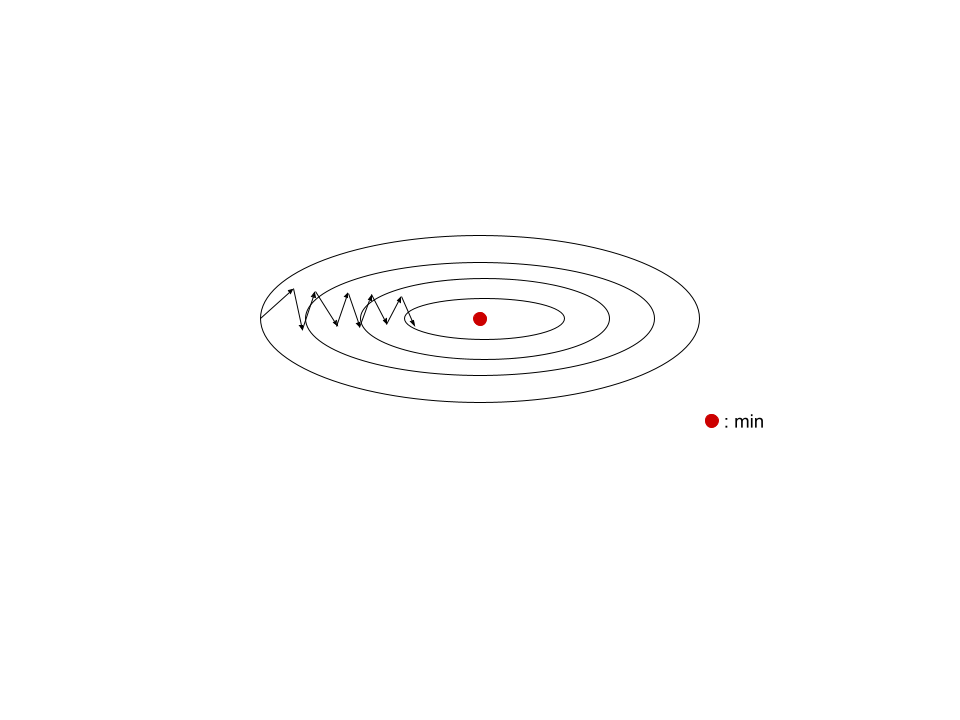
\includegraphics[width=\linewidth]{Figures/Fig1.png}
  \setlength{\abovecaptionskip}{-102pt}  
  \setlength{\belowcaptionskip}{-5pt}
  \caption{Example of Gradient Descent without Momentum}
  \label{fig:image1}
\end{figure}
\begin{figure}[H]
  \centering
  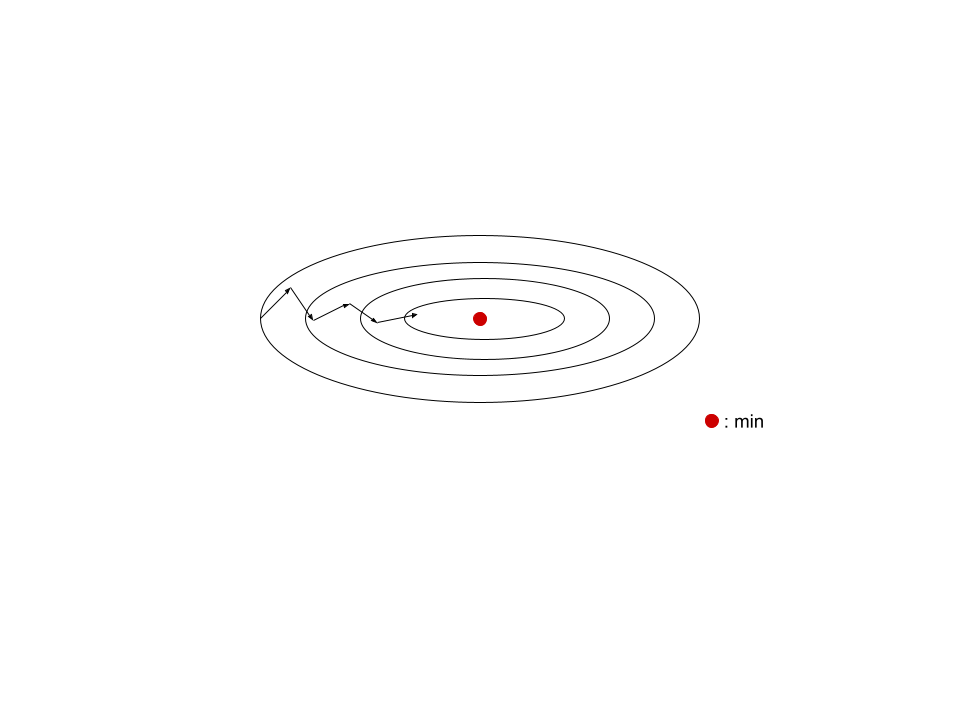
\includegraphics[width=\linewidth]{Figures/Fig2.png}
  \setlength{\abovecaptionskip}{-102pt}  
  \setlength{\belowcaptionskip}{-5pt}
  \caption{Example of Gradient Descent with Momentum}
  \label{fig:image1}
\end{figure}

An intuitive interpretation for Figures 1 and 2 is that if the contours depict elevation within a neighborhood of a surface in $\mathbb{R}^3$, then the fluctuations along directions perpendicular to the z-axis tend to average out to zero, while progress in the z-component is given more weight.

% By taking an exponentially weighted moving average of the gradients, the dominant direction of convergence is taken into, 


\subsection{Problem Statement}
% Discuss the variations of gradient descent methods and their relevance.

\subsection{Research Objectives}
Outline the main objective: to compare stochastic, mini-batch, and batch gradient descent methods in various aspects.

